\documentclass[12pt, a4paper]{article}

\usepackage{graphicx, caption, subcaption, float}     % Figures
\usepackage{minted, xcolor}    % Code
\usepackage{hyperref}    % Links

\renewcommand{\thesubsection}{\alph{subsection}}

\definecolor{cbg}{rgb}{0.95, 0.95, 0.95}

\begin{document}

\begin{titlepage}
\center
\textsc{\LARGE Nanyang Technological University}\\[20mm]
\textsc{\Large CZ4003 Computer Vision}\\[40mm]
\rule{\linewidth}{0.3mm}\\[8mm]
{\huge\bfseries Lab 2}\\[4mm]
\rule{\linewidth}{0.3mm}\\[25mm]
\begin{flushright} \large
Onno \textsc{Eberhard}\\
N1804715F
\end{flushright}~\\[45mm]
{\large \today}
\vfill % Fill the rest of the page with whitespace
\end{titlepage}

\tableofcontents
\newpage

\section{Edge Detection}
\subsection{Load image, transform to greyscale and display}
Input:
\begin{minted}[bgcolor=cbg, fontsize=\footnotesize, mathescape]{octave}
img = imread('maccropped.jpg');
img = im2double(rgb2gray(img));    % Convert to double for easier use

figure
imshow(img)
\end{minted}
Output:
\begin{figure}[H]
	\centering
	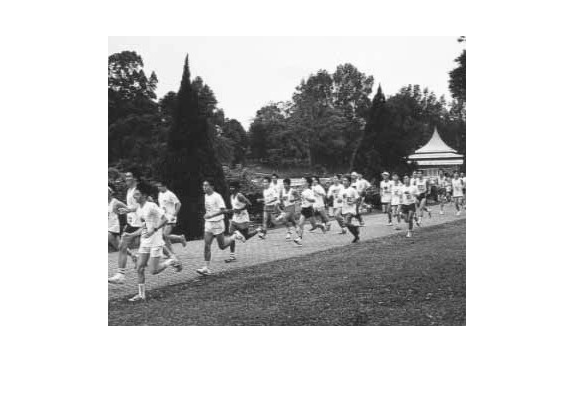
\includegraphics[width=\textwidth]{fig1.png}
\end{figure}
~\\[-15mm]
\subsection{Sobel edge detection}
Input:
\begin{minted}[bgcolor=cbg, fontsize=\footnotesize, mathescape]{octave}
h = [1 2 1; 0 0 0; -1 -2 -1];
v = [1 0 -1; 2 0 -2; 1 0 -1];

edges_h = conv2(img, h);
edges_v = conv2(img, v);

figure
imagesc(edges_h)    % imshow will discard negative values
figure
imagesc(edges_v)
\end{minted}
Output:
\begin{figure}[H]
    \centering %use either centering or hfill (between images)
    \begin{subfigure}[b]{0.45\textwidth}
        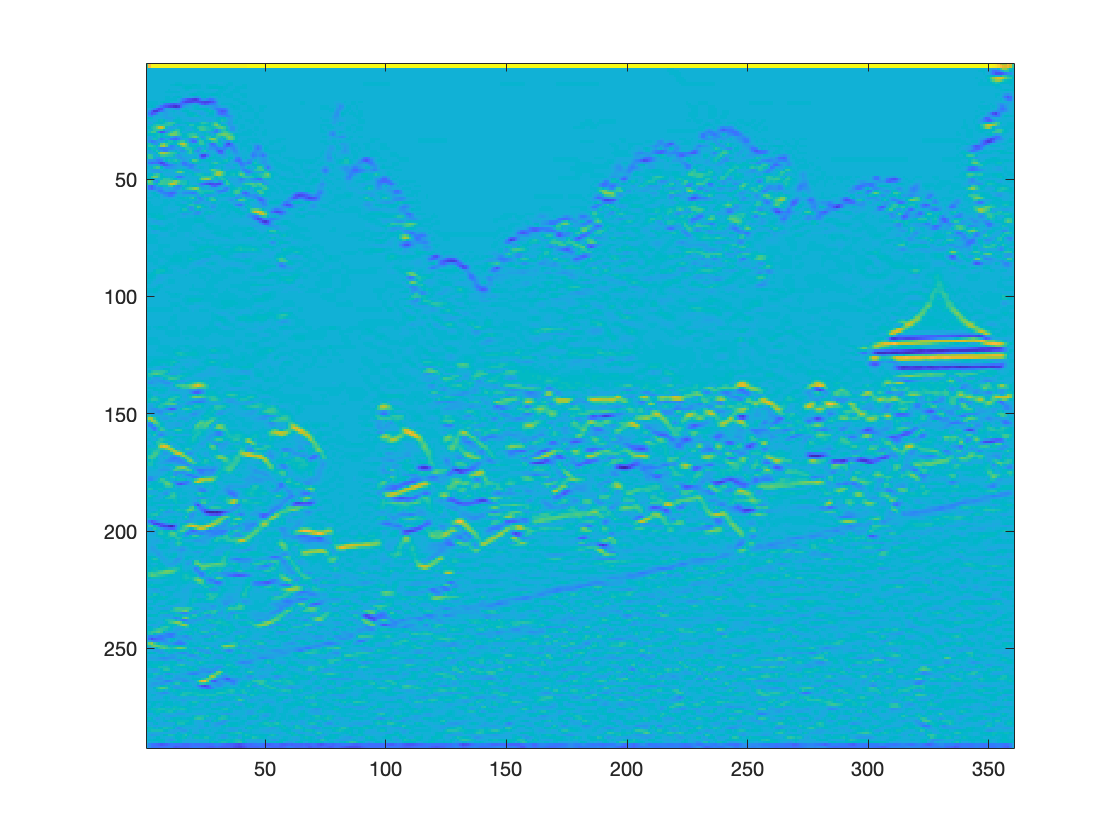
\includegraphics[width=\textwidth]{fig2.png}
        %\caption{Flower one.}
        %\label{fig:f1}
    \end{subfigure}
    %\hfill
    \begin{subfigure}[b]{0.45\textwidth}
        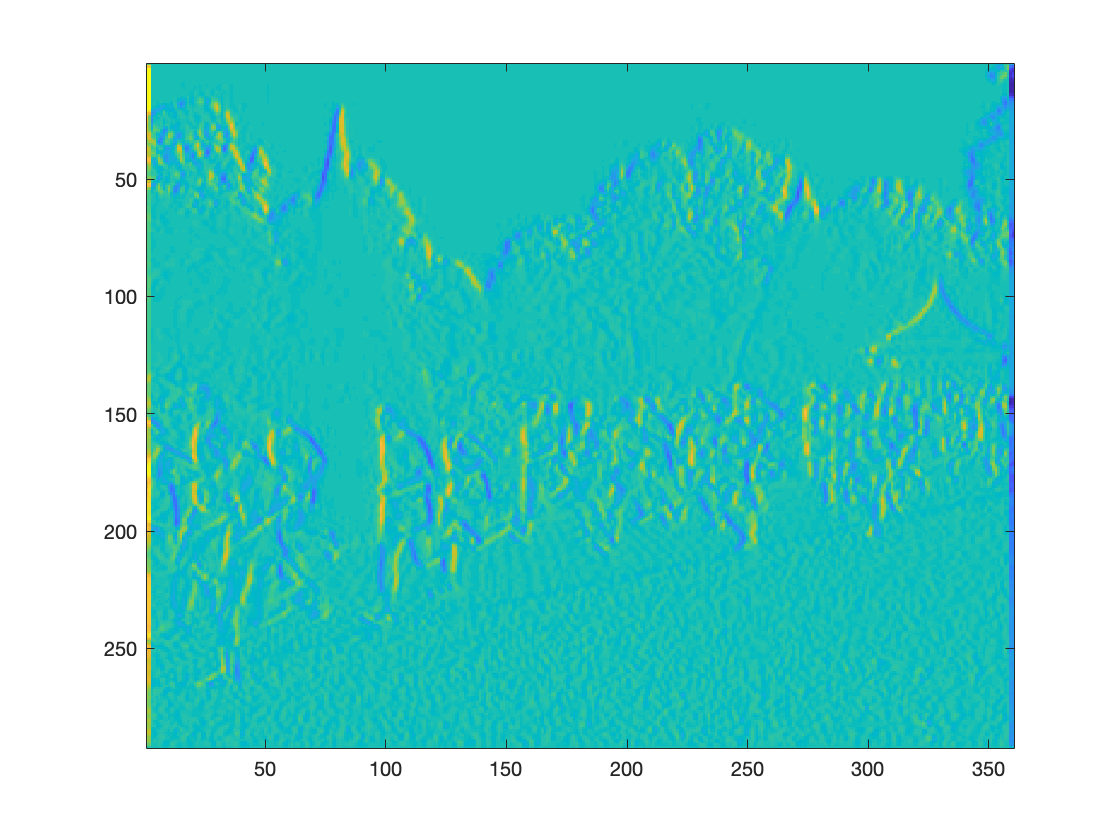
\includegraphics[width=\textwidth]{fig3.png}
        %\caption{Flower two.}
        %\label{fig:f2}
    \end{subfigure}
    %\caption{My flowers.}
\end{figure}
~\\
Diagonal edges mostly get separated into horizontal and vertical components, like the edge of what looks like a pavilion in the right of the image or the tip of the big tree in the front.


\subsection{Combining edges}
Input:
\begin{minted}[bgcolor=cbg, fontsize=\footnotesize, mathescape]{octave}
edges = edges_h.^2 + edges_v.^2;
figure
imshow(edges)

% Getting rid of the edges of the image and normalising
edges = edges(3:end-2, 3:end-2);
edges = edges / max(max(edges));   
figure
imshow(edges)
\end{minted}
\newpage
Output:
\begin{figure}[H]
	\centering
	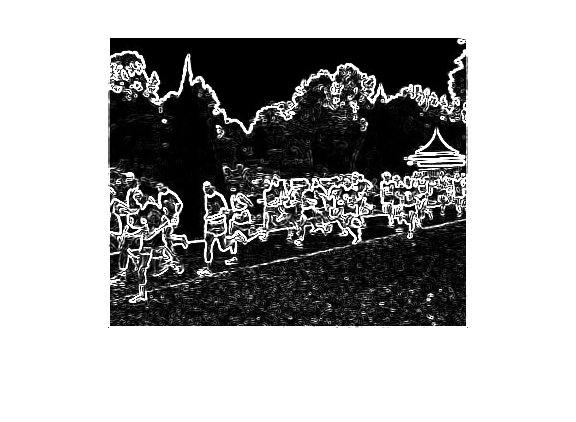
\includegraphics[width=\textwidth]{fig4.png}
\end{figure}
~\\[-20mm]
\begin{figure}[H]
	\centering
	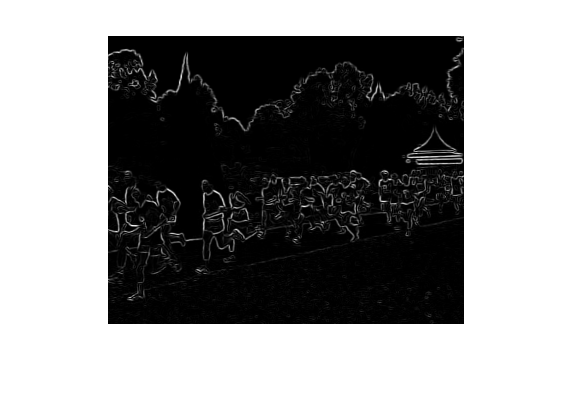
\includegraphics[width=\textwidth]{fig5.png}
\end{figure}
~\\
The squaring will dismiss values that are very small (insignificant) in both filtered images. It will also get rid of the minus sign resulting from Sobel filtering.

\subsection{Thresholding}
Input:
\begin{minted}[bgcolor=cbg, fontsize=\footnotesize, mathescape]{octave}
img_t1 = edges > .1;
img_t2 = edges > .3;
img_t3 = edges > .5;

figure
imshow(img_t1)
figure
imshow(img_t2)
figure
imshow(img_t3)
\end{minted}
Output:
\begin{figure}[H]
	\centering
	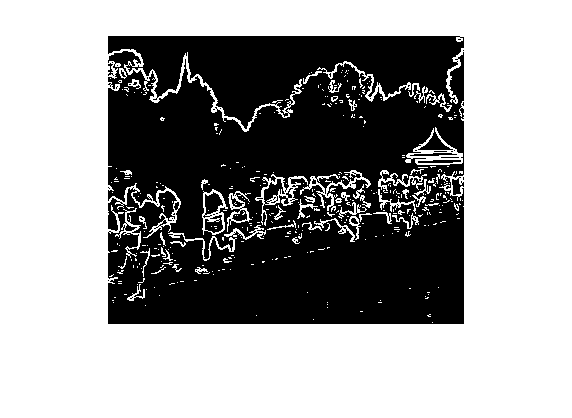
\includegraphics[width=\textwidth]{fig6.png}
\end{figure}
~\\[-20mm]\begin{figure}[H]
	\centering
	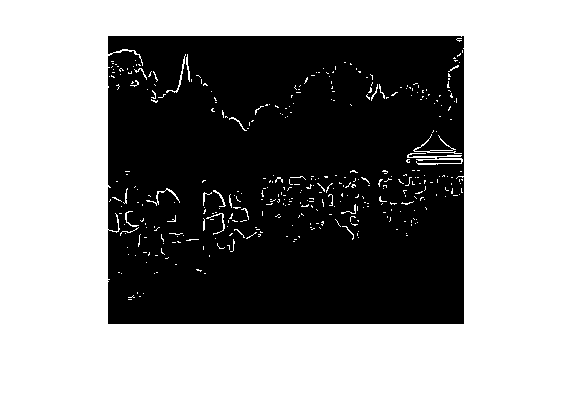
\includegraphics[width=\textwidth]{fig7.png}
\end{figure}
~\\[-20mm]\begin{figure}[H]
	\centering
	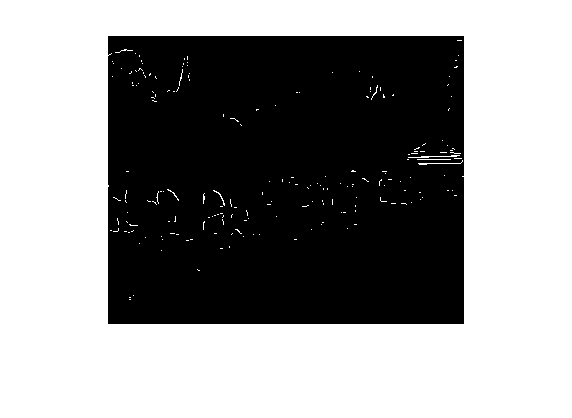
\includegraphics[width=\textwidth]{fig8.png}
\end{figure}
~\\[-20mm]
An advantage of thresholding is that it is very simple, but still often produces acceptable results. It is often important to have a binary image (e.g. as a mask), so tresholding (or similar techniques) are necessary tools in that context. The drawback of thresholding is that it is a very naive technique. Every pixel is processed in the same way and independent of its surroundings. This results in the breaking up of (obvious) edges among other things.\\
Using a small threshold will will not get rid of all noisy non-edge edgels. Using a large threshold will, but it will also break up existing edges into small pieces.


\subsection{Canny edge detection}
Input:
\begin{minted}[bgcolor=cbg, fontsize=\footnotesize, mathescape]{octave}
tl = 0.04;
th = 0.1;
sigma = 1;
E = edge(img, 'canny', [tl th], sigma);
figure
imshow(E)

sigma = 2.5;
E = edge(img, 'canny', [tl th], sigma);
figure
imshow(E)

sigma = 5;
E = edge(img, 'canny', [tl th], sigma);
figure
imshow(E)

sigma = 1; tl = 0.09;
E = edge(img, 'canny', [tl th], sigma);
figure
imshow(E)

tl = 0;
E = edge(img, 'canny', [tl th], sigma);
figure
imshow(E)
\end{minted}
\newpage
Output:
\begin{figure}[H]
	\centering
	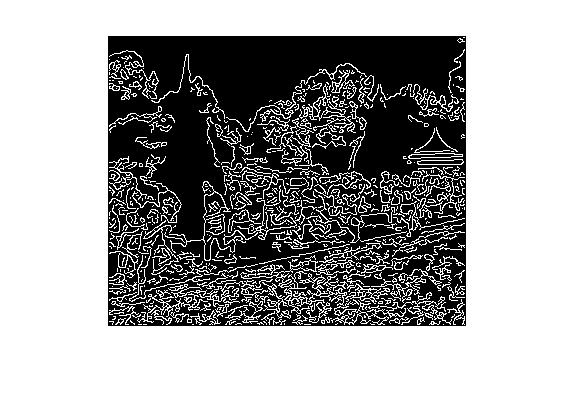
\includegraphics[width=\textwidth]{fig9.png}
\end{figure}
\vspace{-20mm}
\begin{figure}[H]
	\centering
	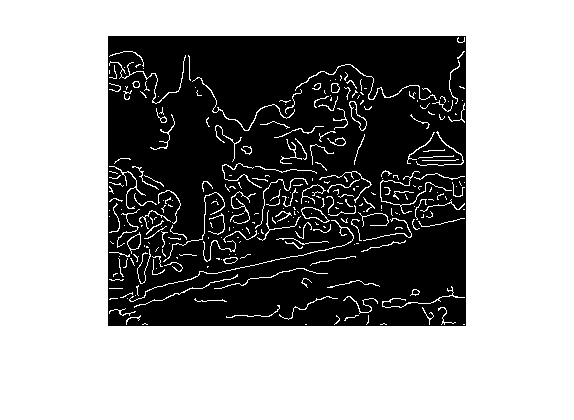
\includegraphics[width=\textwidth]{fig10.png}
\end{figure}
\begin{figure}[H]
	\centering
	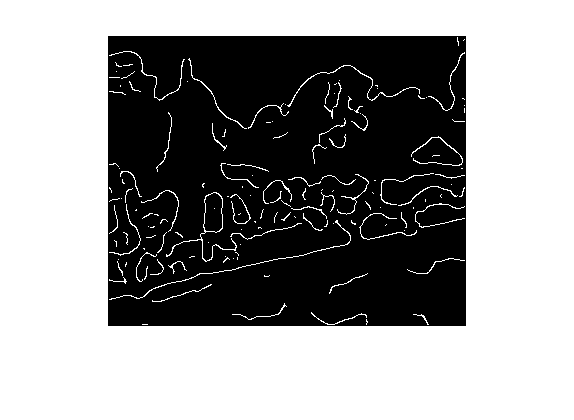
\includegraphics[width=\textwidth]{fig11.png}
\end{figure}
\begin{figure}[H]
	\centering
	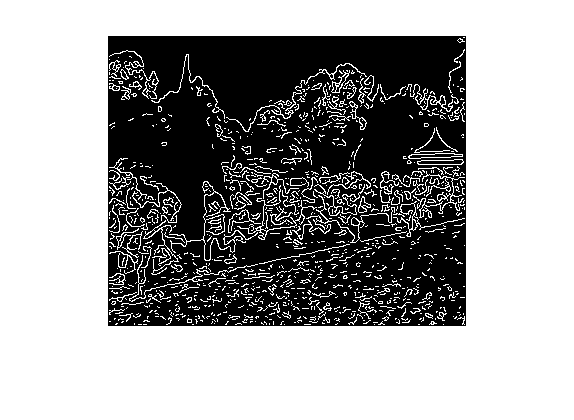
\includegraphics[width=\textwidth]{fig12.png}
\end{figure}
\begin{figure}[H]
	\centering
	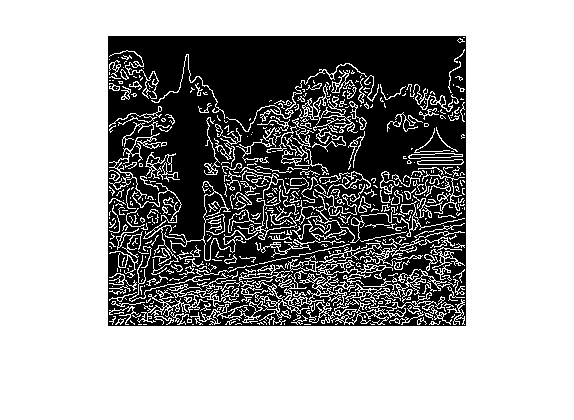
\includegraphics[width=\textwidth]{fig13.png}
\end{figure}
~\\[-20mm]
A lower sigma value corresponds to more noisy, but also more accurate edges. A higher sigma results in fewer and shorter edges, but these are far less accurate. In the sigma = 5 image most shapes have taken on the form of ``blobs'', where no people or trees can be distinguished. The sigma here is the standard deviation of the gaussian kernel with which the image is convoluted. So a higher sigma means very broad, uncertain edges, that never the less get squeezed into one sharp edge; this explains why the high-sigma edges are blob-shaped. A high sigma thus deliveres low location accuracy for the edges, but performs better regarding noise.
Changing the threshold value results in more (lower tl) or less (higher tl) edgels detected.
\newpage
\section{Line Finding using Hough Transform}
\subsection{Canny Edge Detection}
Input:
\begin{minted}[bgcolor=cbg, fontsize=\footnotesize, mathescape]{octave}
tl = 0.04;
th = 0.1;
sigma = 1;
E = edge(img, 'canny', [tl th], sigma);
figure
imshow(E)
\end{minted}
%\newpage
Output:
\begin{figure}[H]
	\centering
	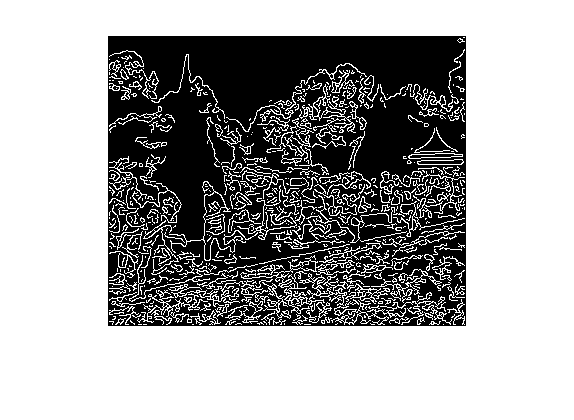
\includegraphics[width=\textwidth]{fig14.png}
\end{figure}

\subsection{Hough Transform}
Input:
\begin{minted}[bgcolor=cbg, fontsize=\footnotesize, mathescape]{octave}
[R, xp] = radon(E);
figure
imagesc(0:179, xp, R)
\end{minted}
%\newpage
Output:
\begin{figure}[H]
	\centering
	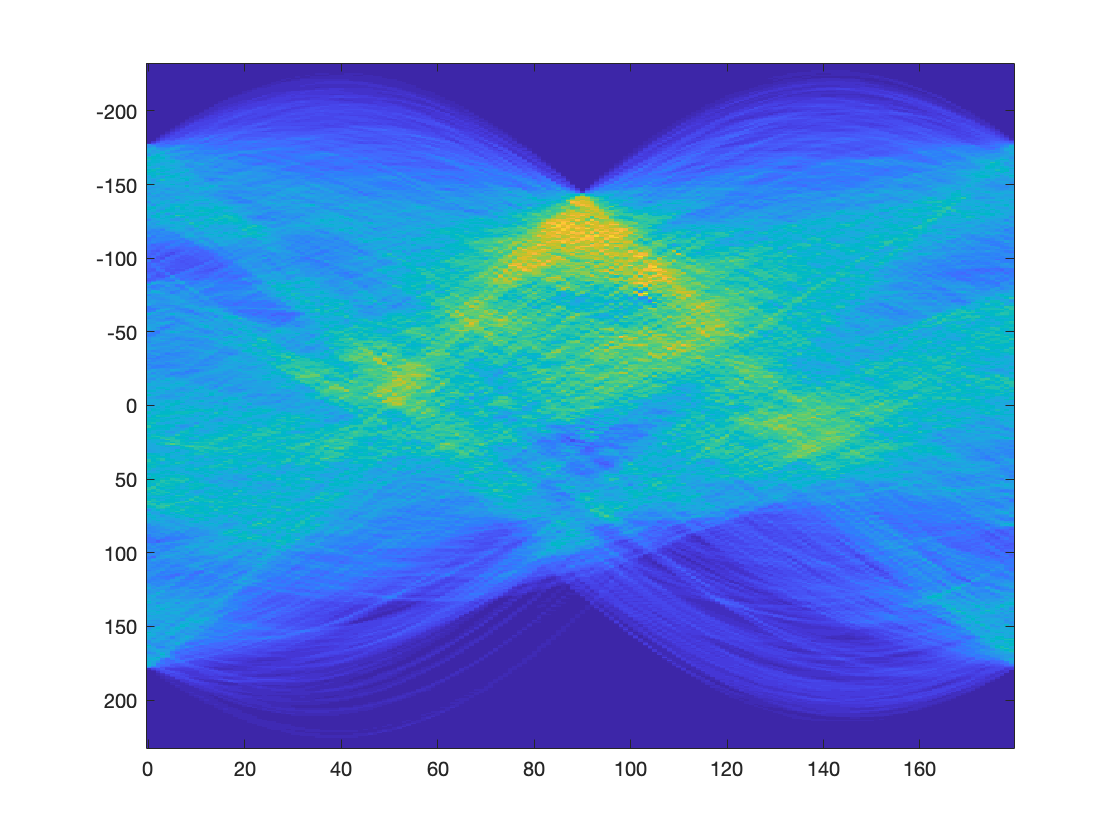
\includegraphics[width=\textwidth]{fig15.png}
\end{figure}

\subsection{Find best line}
Input:
\begin{minted}[bgcolor=cbg, fontsize=\footnotesize, mathescape]{octave}
[i, j] = find(R == max(R(:)));
radius = xp(i);
theta = j * pi / 180;
\end{minted}

\subsection{Transform coordinates}
Input:
\begin{minted}[bgcolor=cbg, fontsize=\footnotesize, mathescape]{octave}
[x0, y0] = pol2cart(theta, radius);
y = @(x) size(img, 1) / 2 - (x0^2 + y0^2 - x0*(x - size(img, 2)/2)) / y0;
\end{minted}
This transforms $r$ and $\theta$ into the same coordinate system used to display the image, so that a line can simply be plotted onto the same surface.
\newpage
\subsection{Display image and line}
Input:
\begin{minted}[bgcolor=cbg, fontsize=\footnotesize, mathescape]{octave}
figure
imshow(img)
hold on
x = linspace(0, size(img, 2));
plot(x, y(x), 'r')
\end{minted}
%\newpage
Output:
\begin{figure}[H]
	\centering
	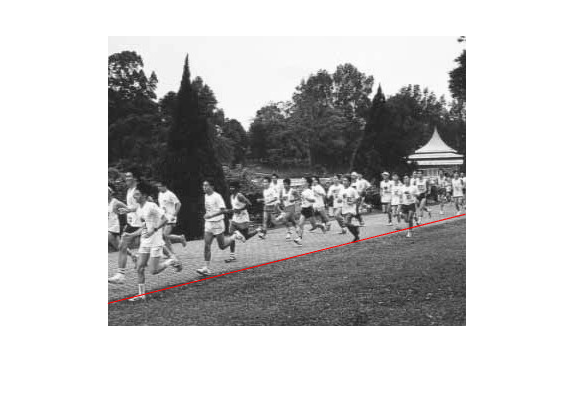
\includegraphics[width=\textwidth]{fig16.png}
\end{figure}
~\\
The line does not perfectly line up with the actual edge of the running path. A good way of improving the result would be to increase the precision of theta for the Hough transform. The position of the line is good enough, but the angle is ever-so slightly off, resulting in a larger error on the edges of the image.

\newpage

\section{3D Stereo}
\subsection{Disparity map algorithm}
\begin{minted}[bgcolor=cbg, fontsize=\footnotesize, mathescape]{octave}
function d = dmap(Il, Ir, th, tw)

[h, w] = size(Il);
d = zeros(h, w);

th_ = floor(th / 2);
tw_ = floor(tw / 2);

for y = th_+1 : h-th_
    for x = tw_+1 : w-tw_
        T = rot90(Il(y-th_ : y+th_, x-tw_ : x+tw_), 2);
        S = conv2(Ir(y-th_ : y+th_, :).^2, ones(th, tw), 'same') ...
            - 2*conv2(Ir(y-th_ : y+th_, :), T, 'same') ...
            + sum(sum(T.^2));
        xr = find(S(tw_+1, :) == min(S(tw_+1, :)), 1);
        d(y, x) = x - xr;
    end
end
\end{minted}

\subsection{Load images}
Input:
\begin{minted}[bgcolor=cbg, fontsize=\footnotesize, mathescape]{octave}
Il = im2double(rgb2gray(imread('corridorl.jpg')));
Ir = im2double(rgb2gray(imread('corridorr.jpg')));
figure
imshow(Il)
figure
imshow(Ir)
\end{minted}
Output:
\vspace{-4mm}
\begin{figure}[H]
    \centering %use either centering or hfill (between images)
    \begin{subfigure}[b]{0.45\textwidth}
        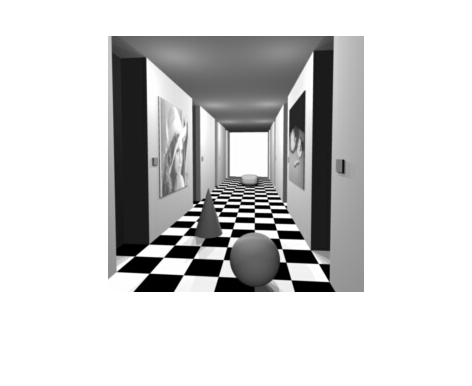
\includegraphics[width=\textwidth]{fig17.png}
        %\caption{Flower one.}
        %\label{fig:f1}
    \end{subfigure}
    %\hfill
    \begin{subfigure}[b]{0.45\textwidth}
        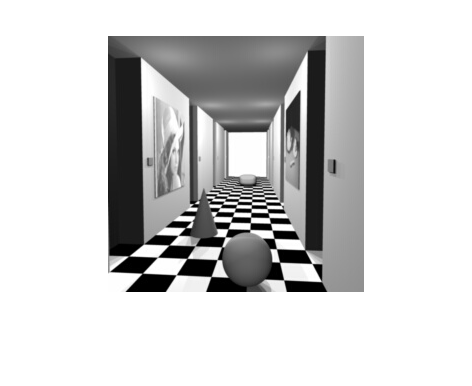
\includegraphics[width=\textwidth]{fig18.png}
        %\caption{Flower two.}
        %\label{fig:f2}
    \end{subfigure}
    %\caption{My flowers.}
\end{figure}

\subsection{Execute algorithm}
Input:
\begin{minted}[bgcolor=cbg, fontsize=\footnotesize, mathescape]{octave}
d = dmap(Il, Ir, 11, 11);
figure
imagesc(d, [-15 15])
\end{minted}
%\newpage
Output:
\vspace{-1mm}
\begin{figure}[H]
	\centering
	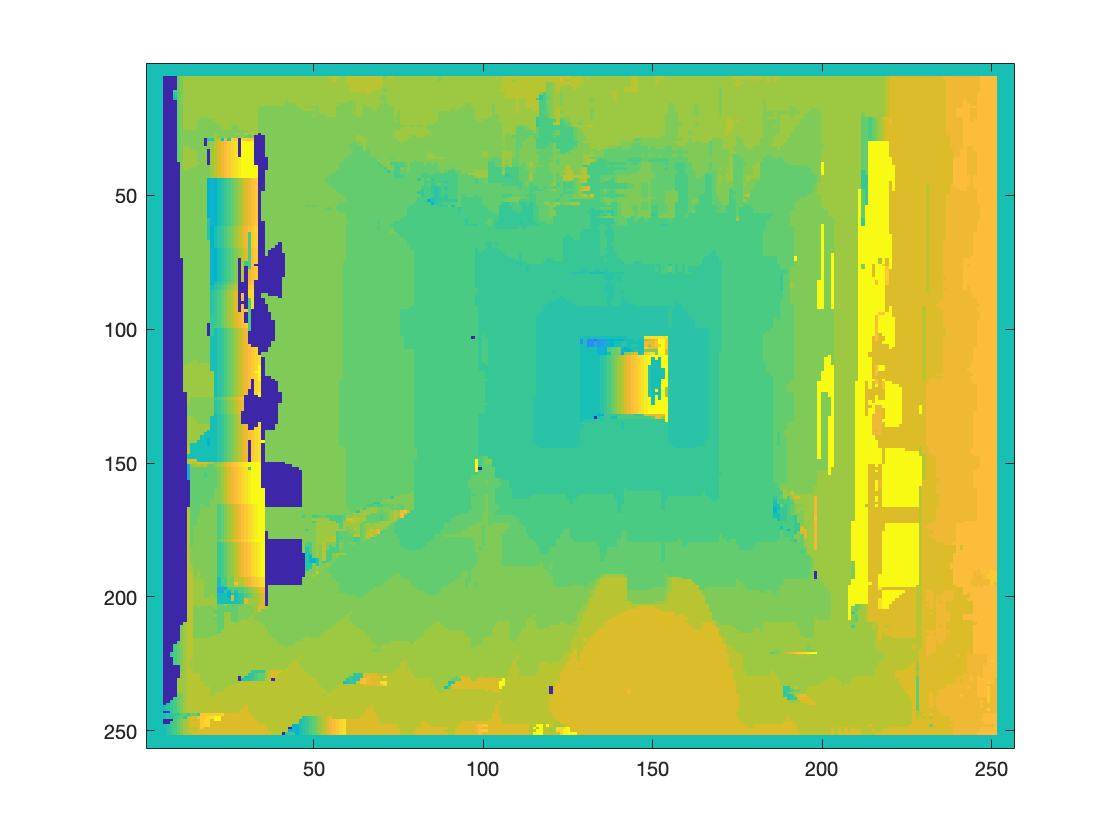
\includegraphics[width=\textwidth]{fig19.png}
\end{figure}
~\\
The disparity is noticeably more accurate in regions where the difference between the image is larger. In the far back, where both images show the same monotonous wall, the algorithm cannot extract the disparity information from the pixels, because they are the same in both images.
\newpage
\subsection{Using real images}
Input:
\begin{minted}[bgcolor=cbg, fontsize=\footnotesize, mathescape]{octave}
Il = im2double(rgb2gray(imread('triclopsi2l.jpg')));
Ir = im2double(rgb2gray(imread('triclopsi2r.jpg')));
figure
imshow(Il)
figure
imshow(Ir)
d = dmap(Il, Ir, 11, 11);
figure
imagesc(d, [-15 15])
\end{minted}
%\newpage
Output:
\begin{figure}[H]
    \centering %use either centering or hfill (between images)
    \begin{subfigure}[b]{0.45\textwidth}
        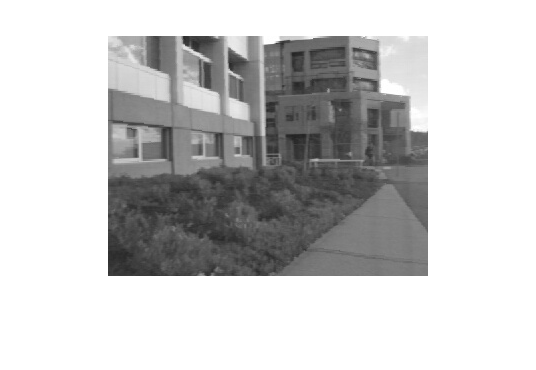
\includegraphics[width=\textwidth]{fig20.png}
        %\caption{Flower one.}
        %\label{fig:f1}
    \end{subfigure}
    %\hfill
    \begin{subfigure}[b]{0.45\textwidth}
        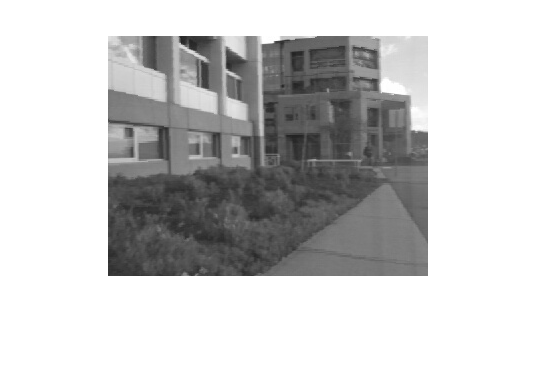
\includegraphics[width=\textwidth]{fig21.png}
        %\caption{Flower two.}
        %\label{fig:f2}
    \end{subfigure}
    %\caption{My flowers.}
\end{figure}
\begin{figure}[H]
	\centering
	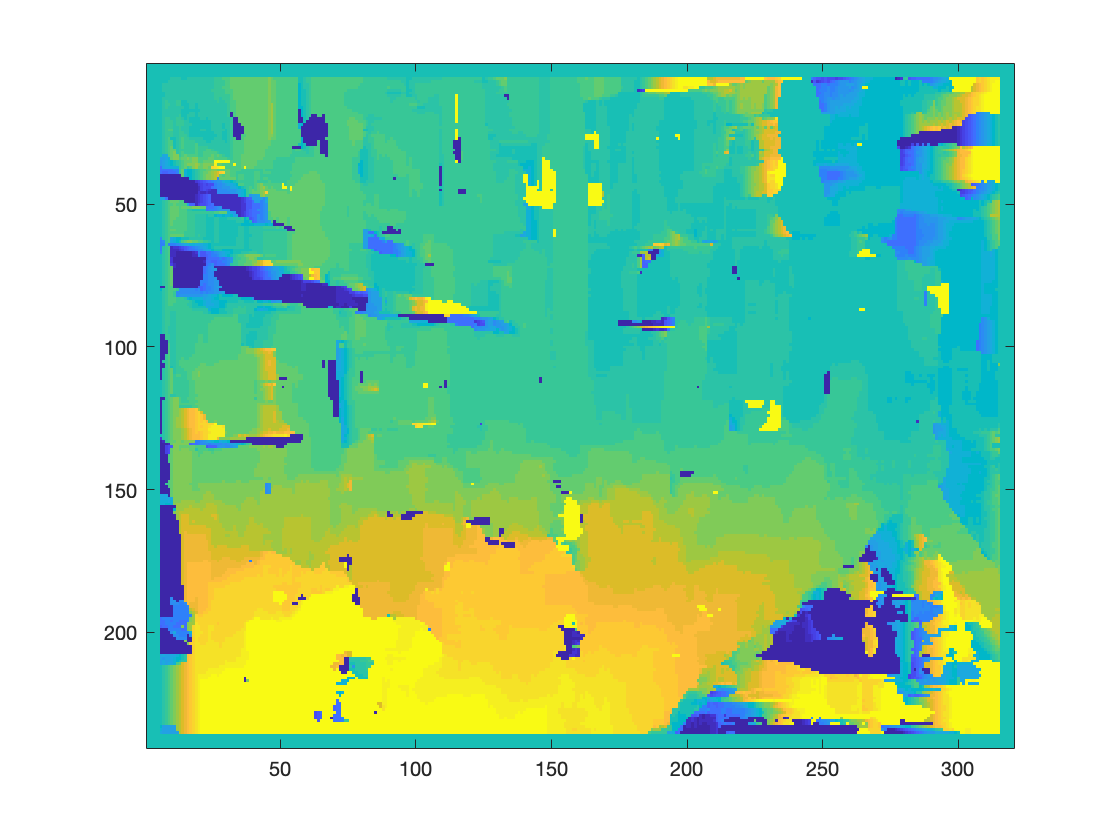
\includegraphics[width=\textwidth]{fig22.png}
\end{figure}
~\\
Again, where the images are more similar (like the facade of the house or the pavement), the disparity is less accurate; the chaotic structure of the bushes makes for significant pixel-by-pixel differences in the images, resulting in high accuracy regarding the disparity. The accuracy also increases if the template size is increased.

\end{document}